% !TEX root = 0000.tex
% Anexo E
% Contenido tomado de main_2.tex (líneas 3972-4039) sin cambios de texto.

% El texto está en inglés: reglas de corte de palabra del inglés
\begin{hyphenrules}{english}

\chapter{Anexo: Error Maps and Training Curves of Experiment 1}\chaptermark{Error Maps of Experiment 1}\label{app:figures}

Each figure shows the pseudo-spectral reference solution, the prediction and the absolute error (top), and
the history of the loss terms during training (bottom).

\begin{figure}[htbp]
  \centering
  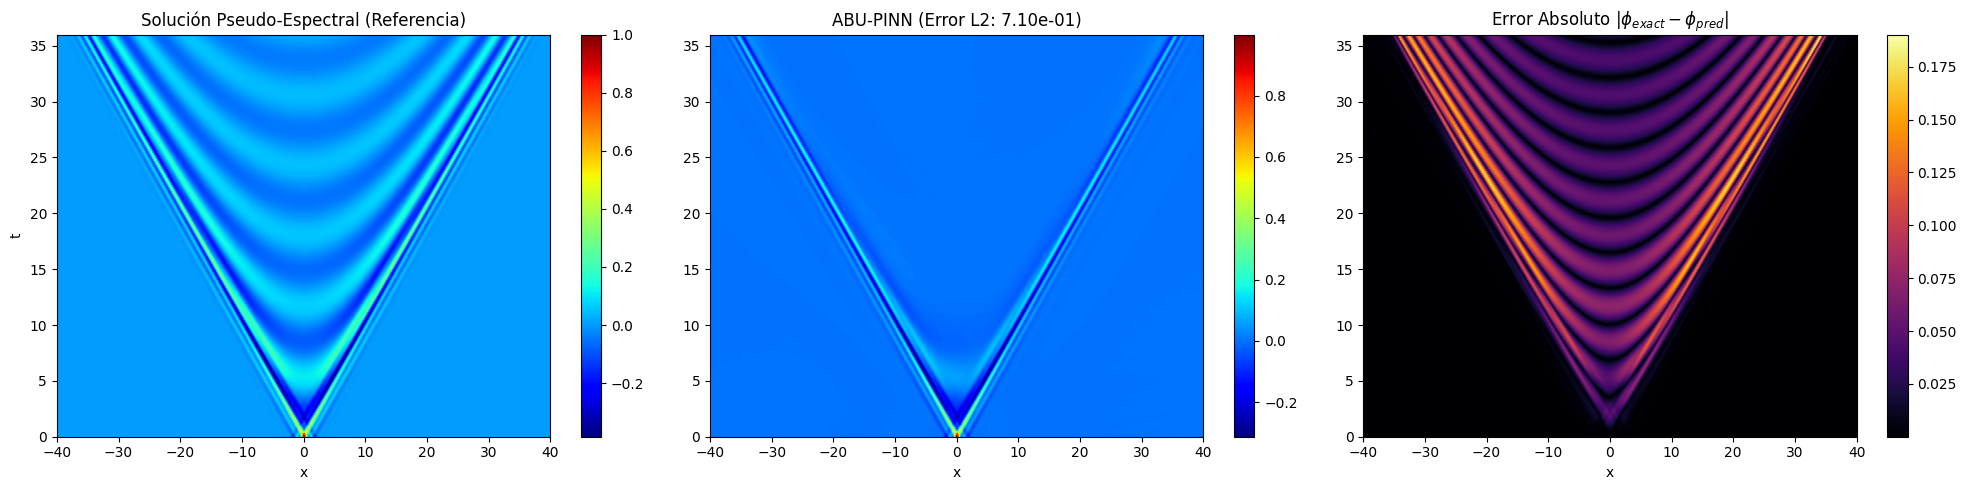
\includegraphics[width=\linewidth]{vanilla_error.png}\\[2mm]
  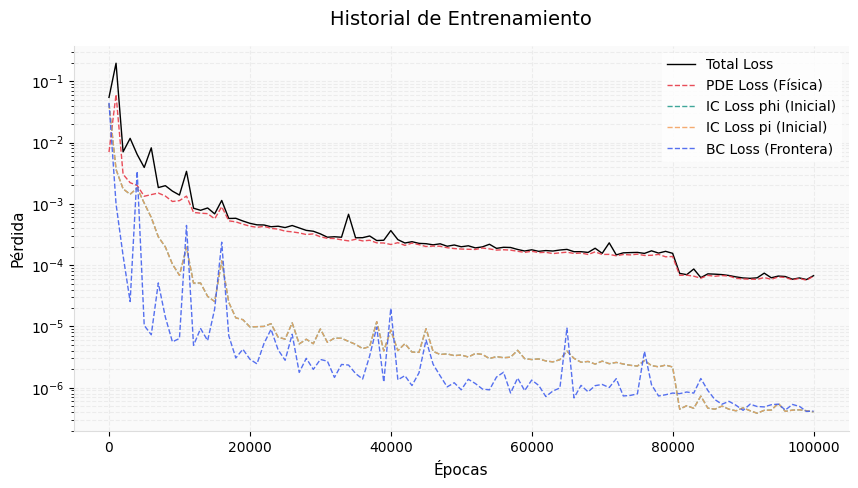
\includegraphics[width=0.55\linewidth]{vanilla_loss.png}
  \caption[Vanilla PINN: error map and training curves]{Vanilla PINN: L2RE 71.0\%. Large errors distributed over the whole region; the total loss oscillates and converges slowly, to values of order $10^{-5}$.}
  \label{fig:app-vanilla}
\end{figure}

\begin{figure}[htbp]
  \centering
  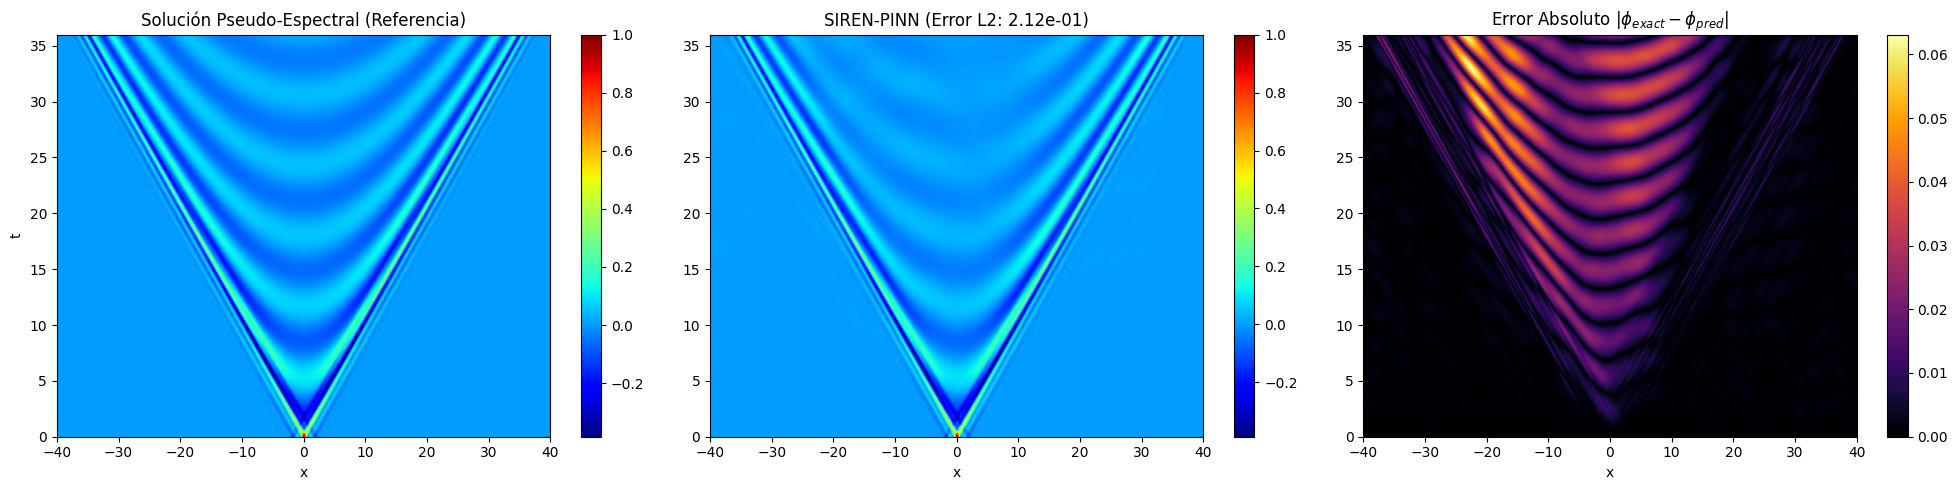
\includegraphics[width=\linewidth]{siren_error.png}\\[2mm]
  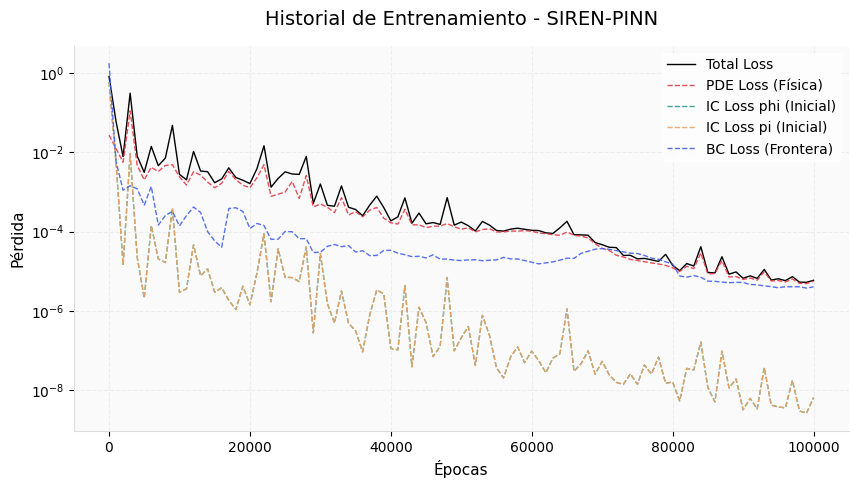
\includegraphics[width=0.55\linewidth]{siren_loss.png}
  \caption[PINN-SIREN: error map and training curves]{PINN-SIREN: L2RE 21.2\%. The maximum errors are reduced with respect to the vanilla PINN, with a better capture of the oscillations; the initial position loss reaches values close to $10^{-8}$.}
  \label{fig:app-siren}
\end{figure}

\begin{figure}[htbp]
  \centering
  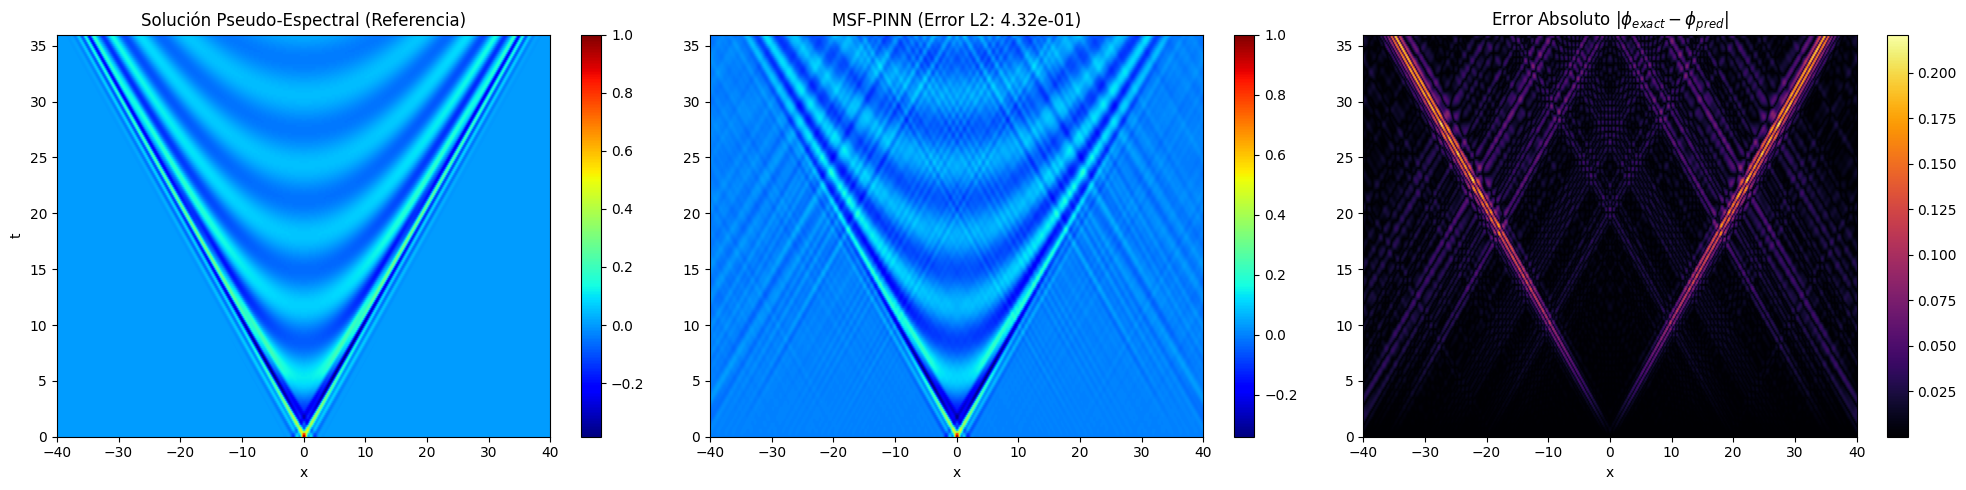
\includegraphics[width=\linewidth]{msf_error.png}\\[2mm]
  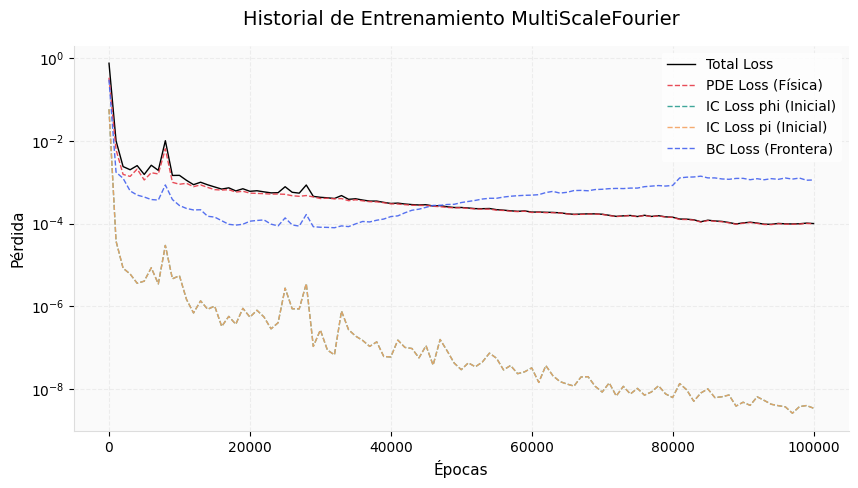
\includegraphics[width=0.55\linewidth]{msf_loss.png}
  \caption[MSF-PINN: error map and training curves]{MSF-PINN: L2RE 43.2\%. Despite the high number of parameters, the errors are significant, especially where the solution has high frequencies; the loss curves show high variance and poor convergence (order $10^{-4}$).}
  \label{fig:app-msf}
\end{figure}

\begin{figure}[htbp]
  \centering
  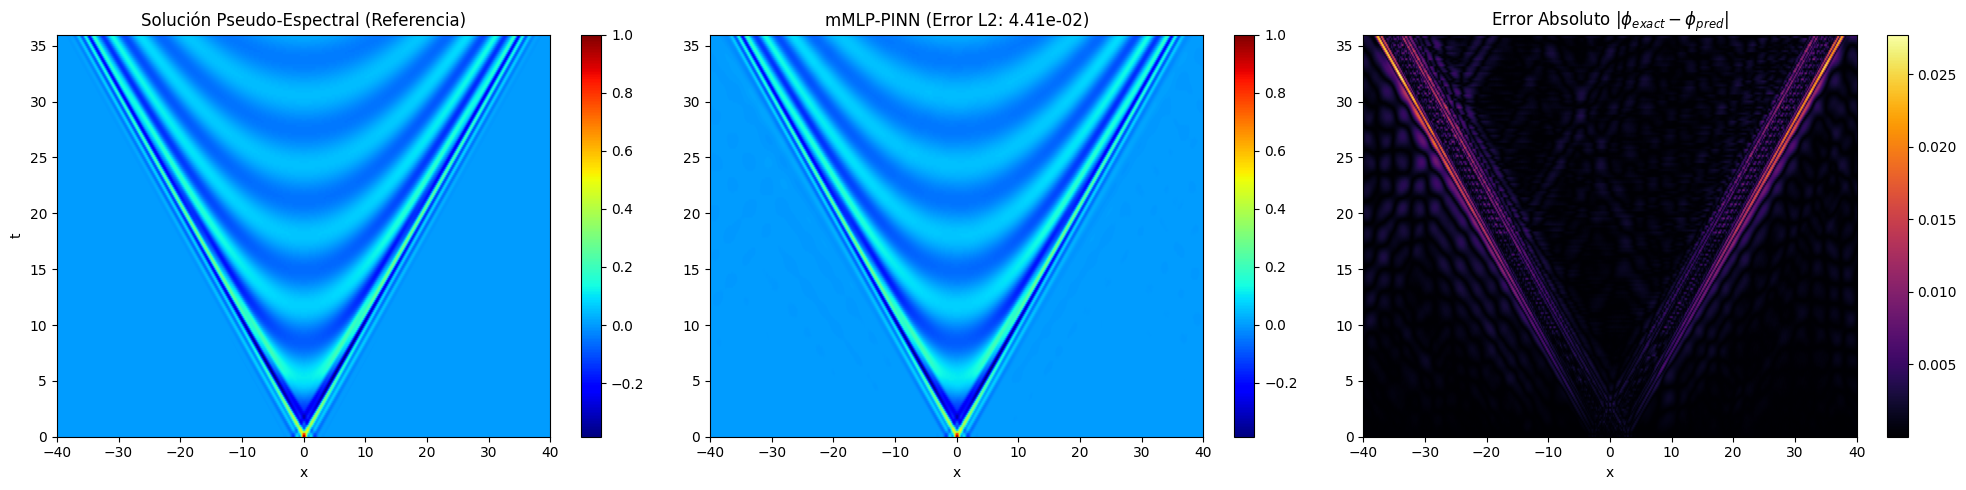
\includegraphics[width=\linewidth]{m4_error.png}\\[2mm]
  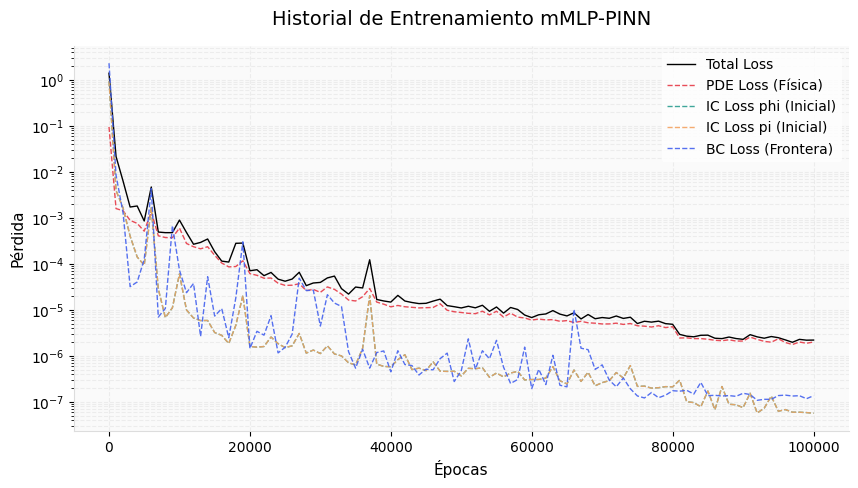
\includegraphics[width=0.55\linewidth]{m4_loss.png}
  \caption[M4-PINN: error map and training curves]{M4-PINN: L2RE 4.41\%. The maximum errors are drastically reduced, with a more homogeneous distribution; the total loss decreases rapidly and stabilizes at about $2.21\times10^{-6}$.}
  \label{fig:app-m4}
\end{figure}

\begin{figure}[htbp]
  \centering
  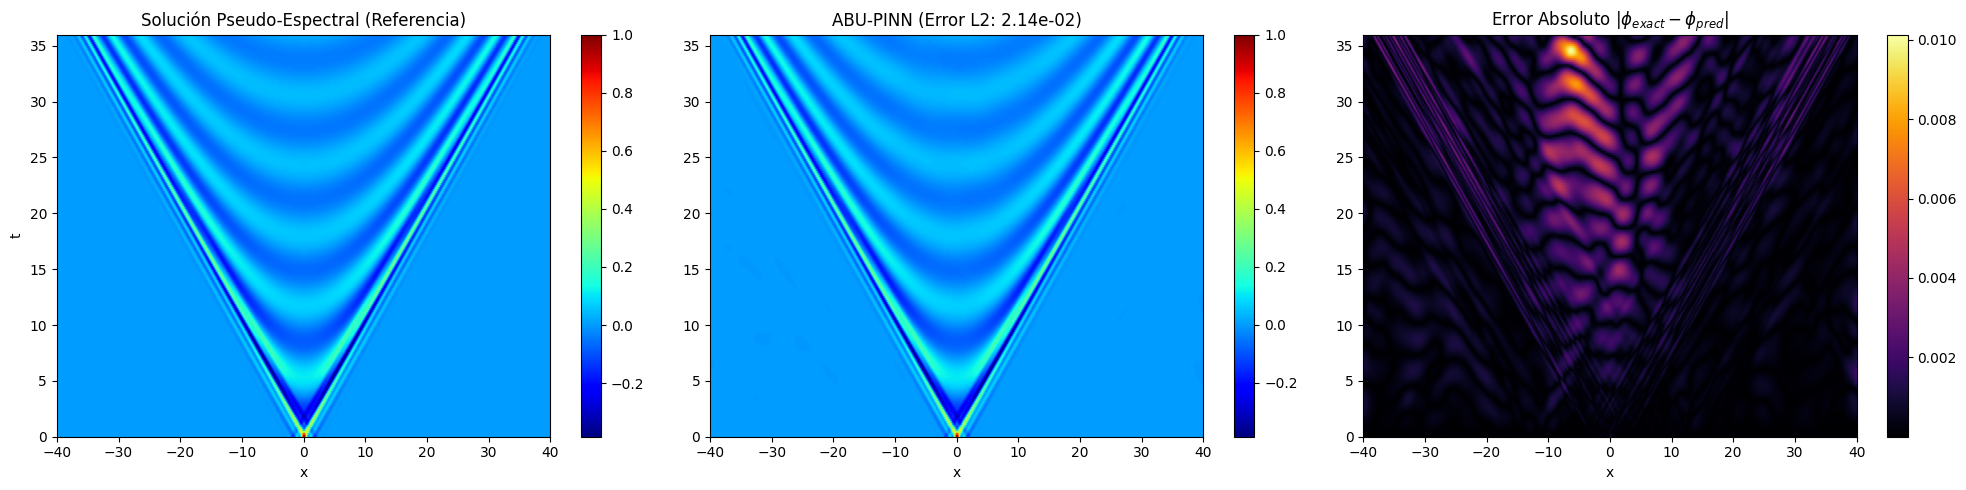
\includegraphics[width=\linewidth]{abu_error.png}\\[2mm]
  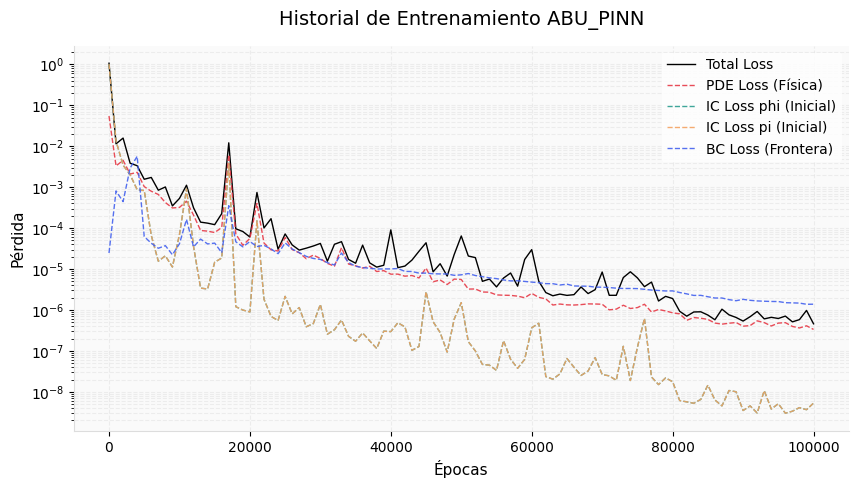
\includegraphics[width=0.55\linewidth]{abu_loss.png}
  \caption[AbuPINN: error map and training curves]{AbuPINN: L2RE 2.14\%. Homogeneous error without pronounced peaks; the total loss reaches $4.60\times10^{-7}$ with an almost stable and fast convergence.}
  \label{fig:app-abu}
\end{figure}

\begin{figure}[htbp]
  \centering
  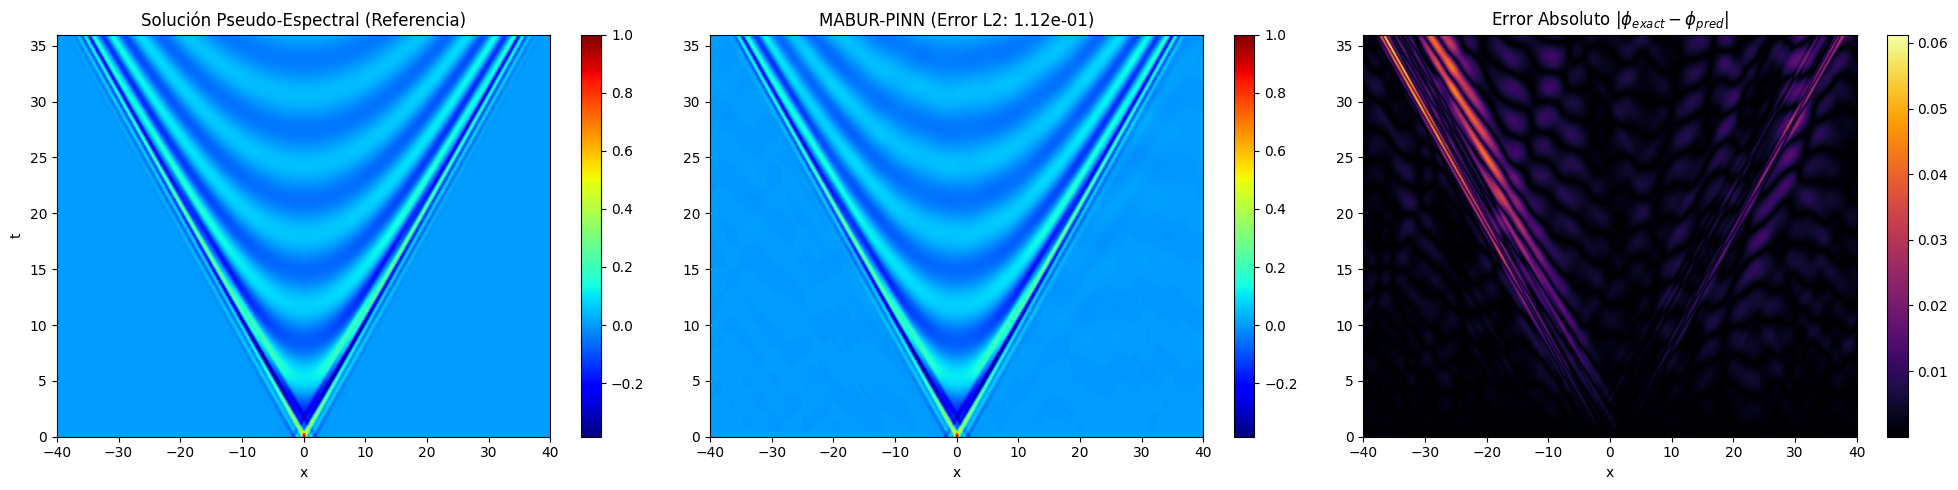
\includegraphics[width=\linewidth]{maburv1_error.png}\\[2mm]
  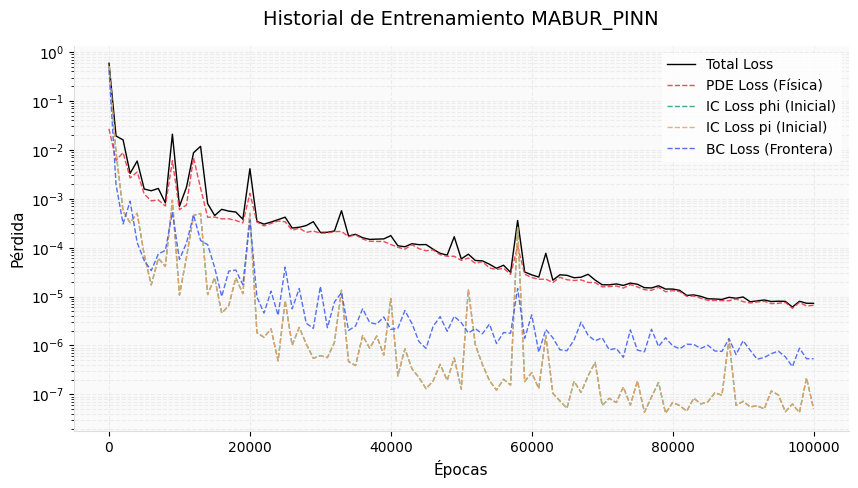
\includegraphics[width=0.55\linewidth]{maburv1_loss.png}
  \caption[MABUR-PINN V1: error map and training curves]{MABUR-PINN V1: L2RE 11.2\%. Improvements in the high-frequency regions with respect to MSF-PINN, but difficulties representing the frequencies inside the light cone; the total loss converges to about $7.25\times10^{-6}$.}
  \label{fig:app-maburv1}
\end{figure}

\begin{figure}[htbp]
  \centering
  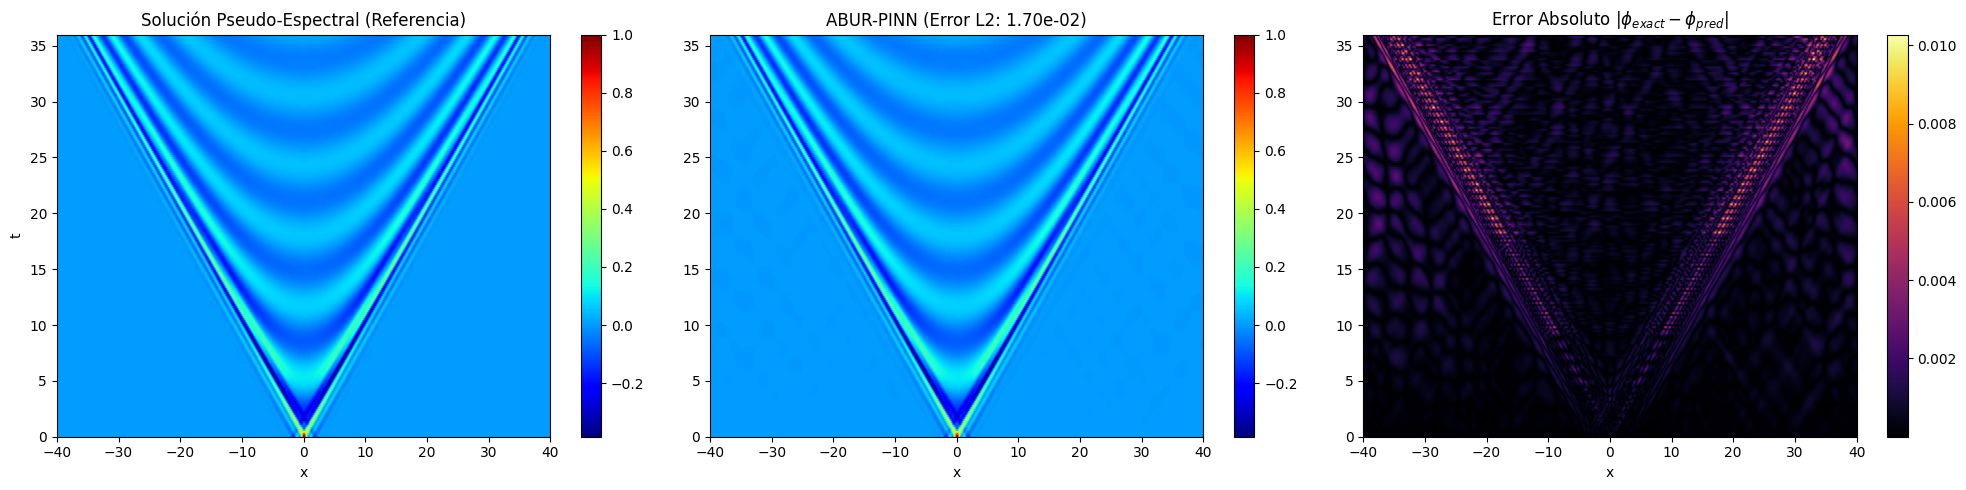
\includegraphics[width=\linewidth]{maburv2_error.png}\\[2mm]
  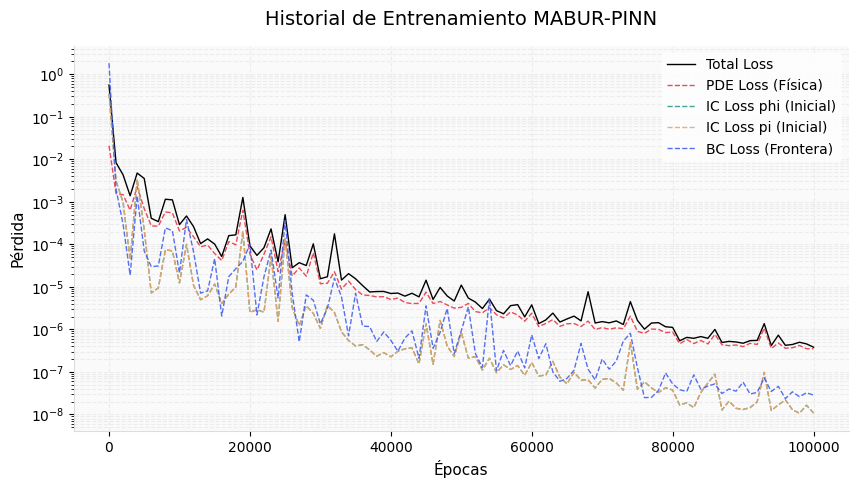
\includegraphics[width=0.55\linewidth]{maburv2_loss.png}
  \caption[MABUR-PINN V2: error map and training curves]{MABUR-PINN V2: L2RE 1.70\%. The error is concentrated on the fronts of the light cone; the total loss converges to $3.81\times10^{-7}$.}
  \label{fig:app-maburv2}
\end{figure}

\begin{figure}[htbp]
  \centering
  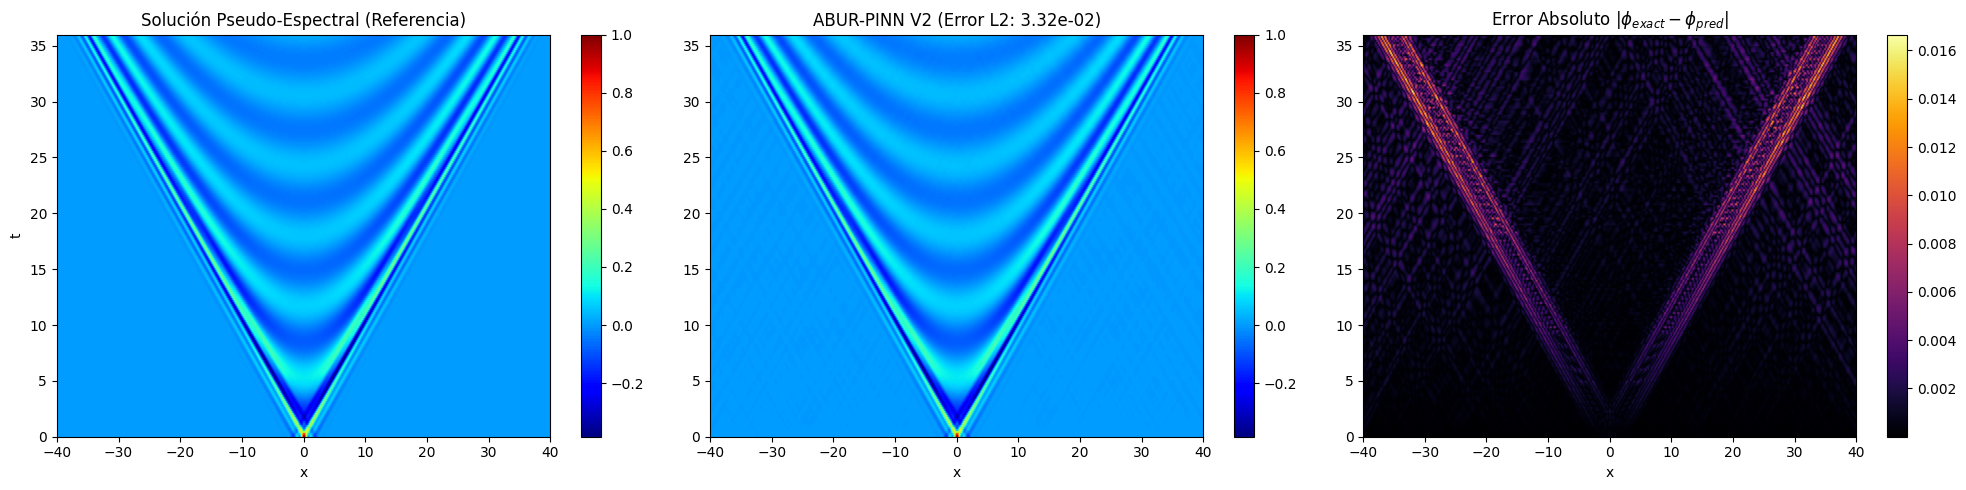
\includegraphics[width=\linewidth]{maburv2_sigma5_error.png}\\[2mm]
  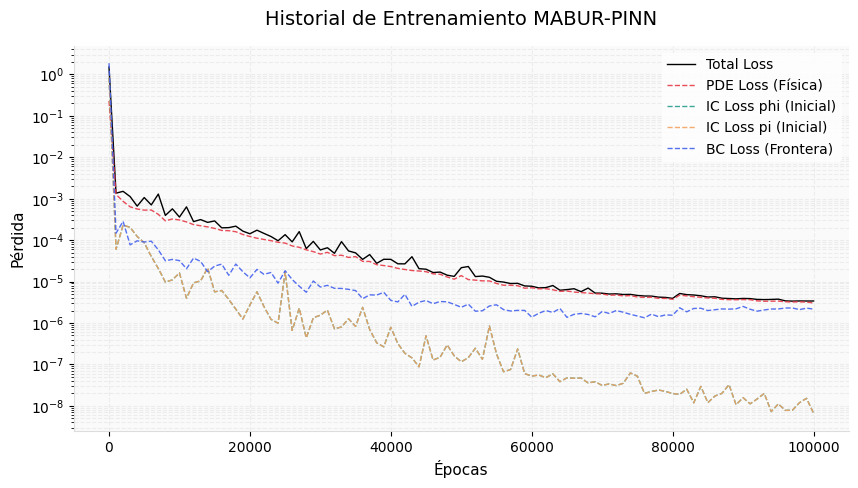
\includegraphics[width=0.55\linewidth]{maburv2_sigma5_loss.png}
  \caption{MABUR-PINN V2 ($\sigma=5$): L2RE 3.32\%. Same architecture with a larger Fourier scale.}
  \label{fig:app-maburv2_sigma5}
\end{figure}

\end{hyphenrules}
